\chapter{Question 2}
\label{question-2}
\section{Question}



\begin{itemize}
\item Use ``Carbon Date'' to estimate the age of each link(s) in a tweet.
	\begin{itemize}
	\item See: http://ws-dl.blogspot.com/2013/04/2013-04-19-carbon-dating-web.html
	\end{itemize}
\item For each t.co link, use ``curl -I -L'' to record the HTTP headers all the way to a terminal HTTP status (i.e. chase down all the redirects)
	\begin{itemize}
	\item Many (most?) deltas will be 0, but there should be many > 0.	
	\end{itemize}
\item For these deltas, compute: median, mean, std dev, std err.	
\item Use wget to download the text for all the links.  Hold on to those, we’ll come back to them later. See:
	\begin{itemize}
	\item \hyperref[savePage]{http://superuser.com/questions/55040/save-a-single-web-page-with-background-images-with-wget}
	\item \hyperref[copyPage]{http://stackoverflow.com/questions/6348289/download-a-working-local-copy-of-a-webpage}
	\end{itemize}
\end{itemize}

\section{Solution}
\begin{itemize}
\item For carbon dating the tweet URI's, I first cloned the github repository.
\item As per the instructions of the author of the library, I then created a bitly account and inserted the accesstoken in the configuration file.
\item Some of the URI's were taking longer than a minute and some a few hours to retrieve the estimated creation date, I split the input files into 1000 URI's each and created five instances of the local.py file with the necessary updates.
\item By splitting these URI's into batches I was able to complete fetching data from each of the URI's in two days.
\item Also, some URI's were stuck for over a few hours and got repeatedly stuck at the same location. I deleted these URI's and continued carbon dating the rest in the list.
\item In the file `local.py' I created a JSON structure with the tweet identifier, creation date of tweet and the estimated creation date of the URI.
\item I used the `getTweetAge.py' for fetching the age of each of these URI's. The figure below indicates the histogram of the Age\textsubscript{tweet} - Age\textsubscript{URI} vs. Frequency.\\*
	\begin{minipage}{\linewidth}
		\centering
		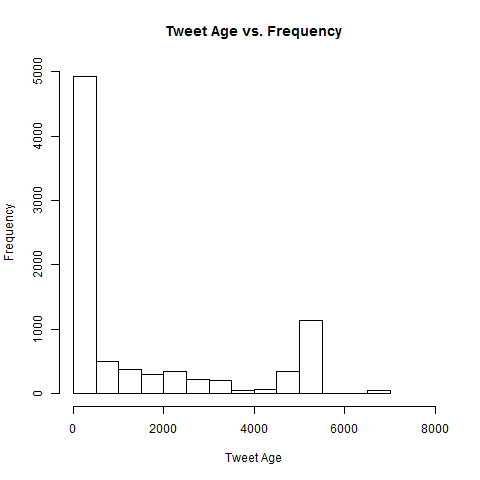
\includegraphics[scale=0.55]{figures/tweetAge.png}
		\captionof{figure}{Age vs. Frequency}
		\label{uriRedirect}
	\end{minipage}
\item Using the age of each of these URI's I found the mean as 1409.735 days, median as 235 days, standard deviation as 1948.022 days, standard error as 21.10941 days.
\end{itemize}
\newpage
\section{Code Listing}
\lstinputlisting[language=Python,breaklines = true,frame=single,caption={Python program for carbon dating the URI's.},label=lst:q1-1,captionpos=b,numbers=left,showspaces=false,showstringspaces=false,basicstyle=\footnotesize]{pythonFiles/local.py}
\newpage
\lstinputlisting[language=Python,breaklines = true,frame=single,caption={Python program for calculating the Age\textsubscript{tweet} - Age\textsubscript{URI}.},label=lst:q1-1,captionpos=b,numbers=left,showspaces=false,showstringspaces=false,basicstyle=\footnotesize]{pythonFiles/getTweetAge.py}
\newpage
\lstinputlisting[language=R,breaklines = true,frame=single,caption={R program for generating the histogram for Age vs. Frequency and calculating mean, median, mode and standard error}, label=lst:q1R1,captionpos=b,numbers=left,showspaces=false,showstringspaces=false,basicstyle=\footnotesize]{rFiles/age.R}